% report.tex

%\documentclass[letterpaper,10pt]{article}
\documentclass[reprint,amsmath]{revtex4-1}


%\usepackage[letterpaper]{geometry}
%\usepackage[font=small]{caption}

\usepackage{hyperref}
\hypersetup{
  bookmarksopen=true,
  pdftitle={QGP parameter extraction via a global analysis of event-by-event flow coefficient distributions},
  pdfauthor={Jonah Bernhard},
}

\usepackage{graphicx}
\graphicspath{{fig/}}

\usepackage{tikz}
\usetikzlibrary{shapes}

%\usepackage[font=small,format=plain,justification=justified]{caption}

\usepackage{short}
\usepackage{deriv}
\usepackage{avg}
\usepackage{unit}
\usepackage{frac}



\begin{document}

\title{QGP parameter extraction via a global analysis \\ of event-by-event flow coefficient distributions}
\author{Jonah Bernhard}
\date{\today}

\maketitle


%\begin{abstract}
%  Heavy-ion collisions produce a hot, dense phase of strongly-interacting matter known as the quark-gluon plasma (QGP) which quickly
%  ($\sim 10^{-23}$ s) expands and freezes into hadrons.  The QGP cannot be observed directly---only final-state hadrons are detectable---so
%  computer models are used to indirectly characterize the medium.  A successful model must simulate realistic collision events and match its
%  final state to experimentally observed particles.
%
%  Modern models use a ``hybrid'' approach with relativistic hydrodynamics for the early hot and dense phase followed by non-equilibrium
%  Boltzmann transport for the dilute hadron-gas phase.  Hybrid models have provided approximate descriptions of a variety of observables, but are
%  very computationally expensive and therefore difficult to test systematically, so they remain poorly constrained.
%
%  One of the most important properties of the QGP is its shear viscosity to entropy density ratio $\eta/s$.  The QGP is postulated to behave
%  as a near-ideal fluid, hence its viscosity may be nearly minimal.  This is explored primarily via collective flow measurements---a natural
%  partner, since viscosity tends to damp collective behavior.  Previous studies have tentatively confirmed a small $\eta/s$, typically by
%  matching the centrality dependence of event-averaged flow coefficients between model and experiment.
%
%  The ATLAS experiment has recently measured event-by-event flow distributions, which could provide a much more sensitive probe
%  of $\eta/s$.  Using a hybrid model with MC-Glauber and MC-KLN initial conditions, viscous 2+1D hydrodynamics, and the hadron cascade UrQMD,
%  we calculate flow distributions over wide ranges of several model parameters including $\eta/s$.  By calibrating the model to data, we
%  extract the optimal values of each parameter and clarify the important features of a physically accurate model.
%\end{abstract}



% 4-8 pages
%  * a broad introduction to the field
%  * the motivation of the topic and contribution to the current status of the field
%  * the methods/techniques used and results that the student may have obtained
%  * a prospective plan for the future


\section{Introduction}


Heavy-ion collisions produce a hot, dense phase of strongly-interacting matter known as the quark-gluon plasma (QGP) which quickly
(${\sim}10^{-23}$ s) expands and freezes into discrete particles.  The QGP cannot be observed directly---only final-state particles are
detectable---so computer models are used to indirectly characterize the medium.  A successful model must simulate realistic collision events
and match its final state to experiment.

Modern models use a ``hybrid'' approach with relativistic fluid dynamics for the early hot and dense phase followed by non-equilibrium
transport for the later dilute gas phase.  Hybrid models have provided approximate descriptions of a variety of observables, but are
very computationally expensive and therefore difficult to test systematically, so they remain poorly constrained.

One of the most important properties of the QGP is its shear viscosity to entropy density ratio $\eta/s$.  The QGP is postulated to behave
as a near-ideal fluid, hence its viscosity may be nearly minimal.  This is explored primarily via collective flow measurements---a natural
partner, since viscosity tends to damp collective behavior.  Previous studies have tentatively confirmed a small $\eta/s$, typically by
matching event-averaged flow between model and experiment.

The ATLAS experiment has recently measured event-by-event flow distributions, which could provide a much more sensitive probe of $\eta/s$.
We systematically test a hybrid model by calculating flow distributions over wide ranges of $\eta/s$ and other salient model parameters and
calibrating to ATLAS data.  This model-to-data comparison will provide optimal values of each parameter---some of which are physical
properties of the QGP---and clarify the important features of a physically accurate model.





\section{Relativistic heavy-ion collisions}


In normal matter, quarks and gluons are confined to composite particles known as hadrons by the strong nuclear force.
The theory which describes these interactions, quantum chromodynamics (QCD), predicts a fluid-like phase of deconfined quarks and gluons at
sufficiently high temperature and density.  This QCD phase is commonly called the quark-gluon plasma (QGP).

It is postulated that the universe was one large QGP in the first microseconds after the Big Bang, before freezing into hadrons.
Similar conditions can be created---on a much smaller scale---in high-energy nuclear collisions.  Simple models of the QGP in such
collisions were proposed forty years ago \cite{chapline}. 

The timescale of relativistic heavy-ion collisions is extremely short, order $10^{-23}$ seconds, and the created matter is correspondingly
small, order $10^{-15}$ meters (1 fm).  Therefore collisions cannot be resolved in time or space; all that can be observed are the
final-state particles which stream into the detector.

Experiments are ongoing at the Relativistic Heavy-Ion Collider (RHIC) at Brookhaven National Lab and the Large Hadron
Collider (LHC) at the European Organization for Nuclear Research.  RHIC collides copper, gold, and uranium nuclei at center of mass energies
up to 200 GeV per nucleon-nucleon pair.  The LHC program performs lead-lead collisions at 2.76 TeV.



\subsection{Spacetime evolution}

\begin{figure*}[t]
  \centering
  \includegraphics[width=\textwidth]{evolution} \\
  0 fm/c   \hspace{.13\textwidth}
  0.5 fm/c \hspace{.13\textwidth}
  8 fm/c   \hspace{.13\textwidth}
  16 fm/c  \hspace{.13\textwidth}
  22 fm/c
  \caption{Schematic evolution of a relativistic heavy-ion collision.  The points in the left frame represent nucleons in colliding nuclei.
    The colored volumes represent QGP, and the red points are hadrons produced in QGP freeze-out.  Figure from \cite{iss}.}
  \label{fig:coll}
\end{figure*}

The dynamics of relativistic boost-invariant nuclear collisions were semi-quantitatively described by Bjorken in 1983 \cite{bjorken}.
Figure \ref{fig:coll} shows a schematic of the spacetime evolution.  In the center of mass frame, nuclei approach each other at (nearly) the
speed of light, Lorentz-contracted into almost-flat discs.  They collide at time $t = 0$, depositing energy and creating new matter in the
process.  This new matter is presumably not initially in thermal equilibrium.  The system has thermalized by time $t \sim 1$ fm/c after the
collision, while the discs recede at the speed of light.  The thermal material (QGP) expands and cools until $t \sim 10$ fm/c, when it
freezes into hadrons.

If one views the collision in a somewhat boosted frame ($\gamma \lesssim 3$), it still looks like a pair of Lorentz-contracted discs
colliding and receding.  This implies approximate boost invariance near mid-rapidity, where spacetime rapidity is defined as
\begin{equation}
  \eta_s = \frac{1}{2} \ln \frac{t + z}{t - z}.
\end{equation}
The central rapidity region ($|\eta_s| \lesssim 3$) contains the hot, dense, fluid-like medium, and most particle production occurs in
central rapidity.  The partner variable to spacetime rapidity is the proper time
\begin{equation}
  \tau^2 = t^2 - z^2,
\end{equation}
which defines hyperbolic surfaces on which the fluid is approximately uniform.


\subsection{Collective behavior and flow}

The QGP is a strongly-interacting fluid-like phase with a very short mean free path, and is therefore expected to exhibit collective
behavior, i.e.\ emitted particles are correlated in phase space.

\begin{figure}[b]
  \centering
  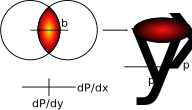
\includegraphics{ellipticflow}
  \caption{Development of elliptic flow in a peripheral collision.  The asymmetric overlap region creates a pressure gradient anisotropy
    $dP/dx > dP/dy$, which drives fluid flow in the $x$-direction.}
  \label{fig:peripheral}
\end{figure}

Ollitrault showed that anisotropies in transverse momentum distributions are an unambiguous signal of transverse collective flow
\cite{ollitrault}.  Consider a peripheral collision of two disc-like nuclei where the impact parameter is large enough that the overlap
region is an asymmetrical almond shape, as in Fig.\ \ref{fig:peripheral}.  This creates a larger pressure gradient along the direction of
the impact parameter---the reaction plane.  This causes the system to expand more quickly in the reaction plane, converting the
initial-state spatial anisotropy into final-state momentum anisotropy.

The efficiency of this position-to-momentum space conversion depends primarily on the shear viscosity of the fluid.  A small shear viscosity
corresponds to a strongly-interacting system with a small mean free path; a large viscosity means strong dissipative effects and damped
collective behavior.  The effect of viscosity is demonstrated in Fig.\ \ref{fig:ichydro}.  QGP viscosity is conventionally expressed as a
dimensionless ratio of the shear viscosity to the entropy density, $\eta/s$.

Anisotropic flow is parameterized by decomposing the transverse-momentum distribution into its Fourier components:
\begin{equation}
  \td N \phi = \frac{N}{2\pi} \biggl\{ 1 + \sum_n v_n \cos [ n(\phi - \Psi) ] \biggr\},
\end{equation}
where $\phi$ is the azimuthal angle of transverse momentum, $\Psi$ is the reaction-plane angle, and the $v_n$ are the flow coefficients.
Each $v_n$ describes the magnitude of the $n$th-order momentum anisotropy:  $v_2$ corresponds to elliptic flow, $v_3$ to triangular flow,
etc., as in Fig.\ \ref{fig:fourier}.

The observation of collective flow provides essential evidence for the existence of a strongly-interacting QCD phase.  Such behavior is a general property of
strongly-interacting systems, ranging from the QGP to an ultra-cold degenerate Fermi gas \cite{fermi}.

\begin{figure}[b]
  \centering
  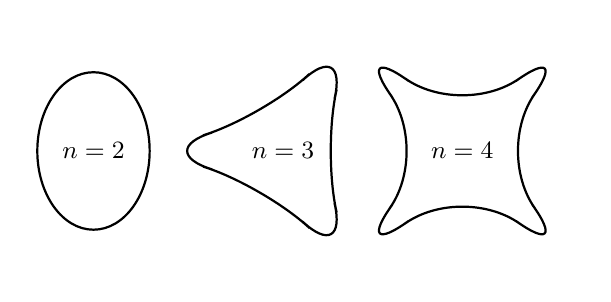
\begin{tikzpicture}
      \small
      \matrix[nodes={draw,thick}] {
        \node[ellipse,minimum height=20mm] {$n=2$}; &
        \node[star, star points=3, rounded corners=8mm, minimum size=10mm, star point ratio=.3,rotate=30] {}; %&
        \node[draw=none] {$n=3$}; &
        \node[star, star points=4, rounded corners=9mm, minimum size=8mm, star point ratio=.2] {$n=4$}; \\
      };
  \end{tikzpicture}
  \caption{Fourier components of flow.}
  \label{fig:fourier}
\end{figure}



\begin{figure*}[t]
  \centering
  \includegraphics{glb-hydro}
  \caption{Left:  Initial condition from the MC-Glauber model for a Pb-Pb collision at 2.76 TeV and $b = 8$ fm.  The initial condition is
    then evolved with viscous hydro.  Middle:  The hydro medium at $\tau = 8$ fm/c with viscosity $\eta/s = 0.04$.  Right:  $\eta/s = 0.24$.}
  \label{fig:ichydro}
\end{figure*}

\subsection{Fluctuations}

The circular nuclei depicted in Fig.\ \ref{fig:peripheral} represent an average over many events.  In this average scenario, the elliptic
flow $v_2$ dominates due to asymmetric overlap, but higher-order even coefficients ($v_4$, $v_6$, \ldots) are much smaller and all odd-order
flows ($v_3$, $v_5$, \ldots) vanish.

More realistic collisions have randomly distributed nucleons and irregular overlap regions, e.g.\ as in Fig.\ \ref{fig:ichydro}.  These
initial-state fluctuations mean that \emph{all} flow coefficients are in general nonzero on an event-by-event level.  $v_2$ will typically
be the largest coefficient for a peripheral collision, since it is driven by systematic initial-state anisotropy, while $v_3$, $v_4$, etc.\
are driven by fluctuations alone.  In a central collision, i.e.\ one with zero impact parameter and maximal overlap, all flows including
$v_2$ are caused solely by fluctuations.

Measurement of event-by-event flows provides flow probability distributions $P(v_n)$.  The mean, width, and shape of these distributions are
important probes of QGP properties, notably the viscosity $\eta/s$.




\section{Simulations}

Modern heavy-ion collision simulations employ Monte Carlo (MC) models for the initial state, viscous relativistic fluid dynamics for the hot and
dense stage, and non-equilibrium Boltzmann transport for the late dilute hadron gas phase \cite{bass-dumitru,nonaka-bass,song}.


\subsection{Initial conditions}

An event is initialized by a randomly generated energy or entropy density profile.  The MC-Glauber model \cite{glauber} is the simplest:  it first randomly
samples nucleon positions, then calculates energy or entropy density in the plane transverse to the beam based on the overlap between
colliding nucleons.  The Glauber model produces energy density from both binary collisions (direct interactions between pairs of nucleons)
and wounded nucleons (any participating nucleon).  A parameter $\alpha$ sets the wounded nucleon / binary collision mixture as
$\frac{1}{2}(1-\alpha)\text{WN} + \alpha\,\text{BC}$.
Figure \ref{fig:ichydro} shows a sample initial condition generated by the Glauber model.

The MC-KLN model \cite{kln} samples nucleon positions (as in Glauber) and calculates the nucleon densities in each nucleus.  The local
saturation scale $Q_s$ is determined and used to calculate the gluon distribution functions.  The resulting gluon density is then
proportional to energy density.  The energy and momentum dependence of $Q_s$ is set by a parameter $\lambda$.



\subsection{Relativistic hydrodynamics}

A hydrodynamics code takes the initial condition input and evolves it until freeze-out.  Typically, the pre-equilibrium phase is ignored,
and the initial condition is simply expanded without any interactions until some initial time $\tau_0 \sim 1$ fm/c.

At time $\tau_0$, the medium is assumed to have thermalized, and hydro evolution begins.  Hydro codes solve the conservation equations
\begin{equation}
  \partial_\mu T^{\mu\nu} = 0,
\end{equation}
where
\begin{equation}
  T^{\mu\nu} = (\epsilon + P) u^\mu u^\nu - P g^{\mu\nu} + \pi^{\mu\nu}
\end{equation}
is the stress-energy tensor.  $\epsilon$, $P$, and $u^\mu$ are the energy density, pressure, and flow velocity of the fluid, $g^{\mu\nu}$ is
the metric tensor, and $\pi^{\mu\nu}$ is the shear stress tensor which accounts for dissipation due to viscosity $\eta/s$.  When viscosity
is included, the shear relaxation time $\tau_\Pi$ naturally enters the equations.

An equation of state,
\begin{equation}
  P = P(\epsilon),
\end{equation}
is also required and usually provided by lattice QCD, e.g.\ s95-PCE \cite{eos}.

Some hydro codes reduce computational complexity by  assuming boost-invariance at mid-rapidity and explicitly calculating only the
transverse directions.  ``Time'' is actually the proper time $\tau$, i.e.\ the medium is calculated on proper-time hyperbola.  Such codes
are called 2+1D, meaning two spatial dimensions and time.  Figure \ref{fig:ichydro} shows an example 2+1D hydro calculation.




\subsection{Hadronic freeze-out}

Hydro evolution stops when a pre-specified criterion is satisfied, typically when the temperature has cooled to the QCD transition at
$T \sim 165$ MeV.  The medium then freezes into discrete hadrons on a spacetime hypersurface $\sigma$ with spectra given by the Cooper-Frye
formula \cite{cf}
\begin{equation}
  E \frac{dN_i}{d^3p} = \int_\sigma f_i(x,p) \, p^\mu \, d^3\sigma_\mu,
\end{equation}
where $f_i$ is the particle distribution function, $p^\mu$ is the four-momentum, and $d^3\sigma_\mu$ is an infinitesimal piece of the
hypersurface $\sigma$ whose magnitude is the volume of the element and direction is normal to the element.  The subscript $i$ is an
index over particle species.

The Cooper-Frye formula may be integrated directly to yield spectra.  In a hybrid model, it is randomly sampled to produce an ensemble
of particles.


\subsection{Transport}

The particle ensemble is given to a hadronic transport code such as Ultrarelativistic Quantum Molecular Dynamics (UrQMD)
\cite{urqmd1,urqmd2}.  The transport algorithm calculates collisions and decays by solving the Boltzmann equation
\begin{equation}
  \td{f_i(x,p)}{t} = \mathcal C_i(x,p),
\end{equation}
where $f_i$ is the particle distribution function, $\mathcal C_i$ is the collision kernel which describes source terms, and $i$ is an index
over species.  The results from the transport code are analogous to particles which stream into a detector.




\section{Method}

\begin{figure}[b]
  \centering
  \includegraphics{lhs}
  \caption{Left:  four points from a Latin-hypercube sample in two variables $x,y$.  Grid lines are drawn to guide the eye;
  only one point is present in each row and column.  Right:  LHS of 40 points (20 per dimension).}
  \label{fig:lhs}
\end{figure}

\begin{figure}[b]
  \centering
  \small
  \hspace{.65cm} prior \hspace{3.2cm} posterior \\
  \includegraphics[width=.49\columnwidth]{gpr1} 
  \includegraphics[width=.49\columnwidth]{gpr2}
  \caption{Left:  three random functions drawn from a Gaussian process prior.  One is plotted as a series of points, the others have the
    points connected into a curve.  Right:  three random functions drawn from the posterior, i.e.\ the prior conditioned on the observations
    indicated by plus signs.  The shaded band represents $2\sigma$ error bands; notice how the posterior error is small near the observed
    points and large further away.  Figures from \cite{rasmussen}.}
  \label{fig:emu}
\end{figure}


\begin{figure*}[t]
  \centering
  \includegraphics[width=.85\textwidth]{atlas}
  \caption{ATLAS event-by-event flow distributions for $v_2$ (left), $v_3$ (middle), and $v_4$ (right) for several centrality bins.  Error
    bars are statistical errors, bands are systematic uncertainties on the distribution shape, lines are fits to the Rice distribution Eq.\
    \eqref{eq:rice}.  Figure from \cite{atlas-vn2}.}
  \label{fig:atlas}
\end{figure*}

\subsection{Model-to-data comparison}

A generic model-to-data comparison consists of a computer model which requires a set of input parameters and a corresponding set of
experimental data.  The input parameters must be calibrated so that the model optimally reproduces reality.

If the model runs quickly, simple techniques such as Markov chain Monte Carlo (MCMC) may be used.  However, this requires many ($10^6$)
evaluations of the model and hence is not feasible for slower codes.

Heavy-ion collision models are very computationally expensive:  each event requires roughly an hour of CPU time, and at
least $10^3$ events are required for a statistically significant study of event-by-event fluctuations.  Input parameters correlate
with each other and affect multiple observables, so it is not sufficient to calibrate each parameter independently---all must be varied
simultaneously.

A pair of strategies help reduce the required amount of CPU time:
\begin{itemize}
  \item Evaluate the model at a predetermined set of parameter points.
  \item Interpolate between explicitly calculated points.
\end{itemize}

Suppose a certain model has $M$ input parameters which must be calibrated to data.  The simplest set of parameter points is a factorial
design:  select $N$ evenly-spaced values for each parameter and evaluate the model at all possible combinations.  However, this requires
$N^M$ parameter points which grows very rapidly, e.g. 5 parameters with 10 values each needs $10^5$ total points.  This scheme is also prone
to wasted CPU time, since unlikely parameter values will be evaluated many times.

A much more efficient design is achieved via Latin-hypercube sampling (LHS).  LHS is ideal for slowly-varying models, i.e.\ one which
produces similar results for nearby points in parameter space.  A LHS provides randomly sampled parameter points subject to some conditions:
\begin{itemize}
  \item The \emph{minimum} distance between points is \emph{maximized}.
  \item Parameter values are not repeated.
\end{itemize}
This way, the parameter space is optimally filled without wasting CPU time calculating redundant information.  A typical choice for a
Latin-hypercube design is 20 points per dimension, see e.g.\ Fig.\ \ref{fig:lhs}.

Sparse designs may be interpolated by a Gaussian process emulator \cite{rasmussen}.  A Gaussian process (GP) is generalization of a
Gaussian distribution:  instead of drawing random values from a distribution, random functions are drawn from a process.  Gaussian processes
require a covariance function, e.g. the covariance of a one-dimensional GP between two points $x_1,x_2$ could be
\begin{equation}
  \text{cov}(x_1,x_2) \propto \exp \biggl[ -\frac{(x_1-x_2)^2}{\ell^2} \biggr] 
\end{equation}
where $\ell$ is the correlation length, so that nearby points are strongly correlated and distant points are independent.

When used for interpolation, a GP emulator assumes that the model is a generic GP (the prior) and is trained on the Latin-hypercube points
to produce conditioned GPs (the posterior).  The posterior provides a statistical distribution of the model outputs with more certainty
closer to explicitly calculated points, hence, it acts as a fast surrogate to the actual model while reflecting the true state of knowledge.
Figure \ref{fig:emu} shows a generic one-dimensional example.




\subsection{Experimental data}

\def\obs{^\text{obs}}

The ATLAS experiment at the LHC has measured event-by-event flow probability distributions for $v_2,v_3,v_4$ from Pb-Pb collisions at 2.76
TeV \cite{atlas-vn,atlas-vn2}.

Flows are calculated event-by-event as two-dimensional vectors $\vec v_n = (v_{n,x},v_{n,y})$ using the single-particle definition
\begin{equation}
  v_{n,x} = \avg{\cos n\phi}, \quad
  v_{n,y} = \avg{\sin n\phi},
\end{equation}
where the average is over all particles in the event.  The flow coefficients are the vector magnitudes
\begin{equation}
  v_n = |\vec v_n| = \sqrt{v_{n,x}^2 + v_{n,y}^2}.
\end{equation}

The probability distribution of flow vectors is assumed to follow a bivariate Gaussian
\begin{equation}
  P(\vec v_n) = \frac{1}{2\pi\delta_{v_n}^2} e^{ -\frac{(\vec v_n - \vec v_n^\text{RP})^2}{2\delta_{v_n}^2} },
  \label{eq:2dgauss}
\end{equation}
where $\vec v_n^\text{RP}$ is the average flow vector and $\delta_{v_n}$ is the width of fluctuations around the mean.  
The one-dimensional distribution of magnitudes is obtained by integrating out the azimuthal angle in Eq.\ \eqref{eq:2dgauss} and is called
the Rice or Bessel-Gaussian distribution:
\begin{equation}
  P(v_n) = \frac{v_n}{\delta_{v_n}^2} e^{ -\frac{(v_n)^2 + (v_n^\text{RP})^2}{2\delta_{v_n}^2} }
    I_0 \pfrac{v_n^\text{RP}v_n}{\delta_{v_n}^2},
  \label{eq:rice}
\end{equation}
where $I_0$ is the modified Bessel function of the first kind.  ATLAS fits their data to the Rice distribution, thereby reducing each
distribution to two parameters, $v_n^\text{RP}$ and $\delta_{v_n}$.  The Gaussian assumption is excellent for central collisions and
acceptable for peripheral collisions, where the tails fall off somewhat more sharply than a Gaussian.

Observed flow distributions are smeared by finite-multiplicity fluctuations and physical nonflow effects such as jets.  The true
distribution $P(v_n)$ will result in an observed distribution \cite{phobos}
\begin{equation}
  P(v_n\obs) = \int P(v_n\obs|v_n) P(v_n) \, dv_n,
  \label{eq:smear}
\end{equation}
where the response function $P(v_n^\text{obs}|v_n)$ gives the probability of observing flow $v_n^\text{obs}$ from an event with true flow
$v_n$.  ATLAS determines the true flow distribution by measuring the response function directly from the data and iteratively solving Eq.\
\eqref{eq:smear} with a Bayesian unfolding procedure \cite{unfolding}.



\subsection{Computer experiment design}

\begin{table}[b]
  \centering
  \begin{ruledtabular}
  \begin{tabular}{lll}
    Parameter & Glauber & KLN \\
    \hline
    Normalization & 20--60 & 5--15 \\
    $\alpha$ & 0.05--0.30 & --- \\
    $\lambda$ & --- & 0.1--0.3 \\
    $\tau_0$ & \multicolumn{2}{c}{0.2--1.0 fm/c} \\
    $\eta/s$ & \multicolumn{2}{c}{0.0--0.3} \\
    $\tau_\Pi$ & \multicolumn{2}{c}{0.2--1.1 fm/c} \\
  \end{tabular}
  \end{ruledtabular}
  \caption{Input parameter ranges for calibration.}
  \label{tab:params}
\end{table}

Simulated event-by-event flow distributions are calculated with a modern hybrid model using MC-Glauber
\cite{glauber} and MC-KLN \cite{kln} initial conditions, viscous 2+1D hydrodynamics \cite{vish}, a Cooper-Frye
hypersurface sampler \cite{iss}, and UrQMD \cite{urqmd1,urqmd2}.  It is an updated version of the OSU/Duke model VISHNU (Viscous Hydro and
UrQMD) \cite{song}.

A set of the five most salient model parameters is selected for calibration.  The initial condition normalization must be calibrated, though
it is not a physical parameter, since it sets the total amount of entropy deposited in a collision.  For the Glauber model, the wounded
nucleon / binary collision parameter $\alpha$ is varied; for KLN, the saturation scale exponent $\lambda$ is chosen.  The variable hydro
parameters are the thermalization time $\tau_0$, specific shear viscosity $\eta/s$, and shear relaxation time $\tau_\Pi$.  Table
\ref{tab:params} summarizes the parameters.

Parameter points are generated from a 256-point five-dimensional Latin hypercube.  The initial goal is 1000 events per design point, in the
centrality bins 0--5\%, 5--10\%, \ldots, 50--55\%, and both Glauber and KLN models, for a total of 3 million events.  At roughly one hour
per event, this represents over 300 years of CPU time.  Events are run in parallel on the Open Science Grid (OSG), which can execute $10^4$
events simultaneously and provide $10^5$ CPU hours per day.

The event-by-event model and all utilities for running on the OSG are publicly available at \url{https://github.com/jbernhard/ebe-osg}.
This package automates running batches of events on the OSG with easy tuning of input parameters.  Results are copied directly from OSG
machines to storage space at Duke.


\subsection{Data analysis}

Observed flows are calculated from UrQMD output using the same single-particle method as ATLAS; $v_n^\text{RP}$ and $\delta_{v_n}$ are then
extracted via a maximum-likelihood fit to the Rice distribution.  Finite-multiplicity smearing still must be removed, but unlike the
experimental distributions, the ``detector'' is perfectly efficient and nonflow effects are absent.  The response function results from pure
Gaussian statistical smearing, hence it is another Rice distribution:
\begin{equation}
  P(v_n^\text{obs}|v_n) = \frac{v_n^\text{obs}}{\delta_{v_n}^2} e^{ -\frac{(v_n^\text{obs})^2 + (v_n)^2}{2\delta_{v_n}^2} }
    I_0 \pfrac{v_nv_n^\text{obs}}{\delta_{v_n}^2}
\end{equation}
where the width depends only on the multiplicity $M$ as \cite{ollitrault,phobos,atlas-vn2}
\begin{equation}
  \delta_{v_n}^2 = 1/2M.
\end{equation}
Since both the true flow distribution and the statistical smearing are Gaussian, the observed distribution will be yet another Rice
distribution:
\begin{equation}
  P(v_n^\text{obs}) = \frac{v_n^\text{obs}}{(\delta_{v_n}^\text{obs})^2} e^{ -\frac{(v_n^\text{obs})^2 +
  (v_n^\text{RP})^2}{(\delta_{v_n}^\text{obs})^2} } I_0 \pfrac{v_n^\text{RP}v_n^\text{obs}}{(\delta_{v_n}^\text{obs})^2}
\end{equation}
where $v_n^\text{RP}$ is unaffected by the smearing but the width is increased as
\begin{equation}
  (\delta_{v_n}^\text{obs})^2 = \delta_{v_n}^2 + 1/2M.
\end{equation}
Hence, finite-multiplicity effects may be removed by reducing the value of $\delta_{v_n}$ from the maximum-likelihood fit according to the
multiplicity.

The code used to analyze all model output is publicly available at \url{https://github.com/jbernhard/ebe-analysis}, though it is still a
work in progress.



\begin{figure*}[t]
  \centering
  \includegraphics{scatters}
  \caption{Dependence of flow distribution parameters on model parameters for $v_2$ in the 20--25\% centrality bin using the Glauber initial
  condition model.  Scatterplots are model output, black lines are trendlines to guide the eye, and red lines denote the
  experimental ATLAS values.}
  \label{fig:scatters}
\end{figure*}

\section{Results}

The initial batch of OSG events is complete, with 1000--2000 events for each combination of parameter point, centrality class, and
initial condition model, for a total of 3.5 million events.  Assuming a Pb-Pb cross section of 7.65 barn, this equates to an integrated
luminosity of $\sim 0.5 \; \mu\text b^{-1}$ (ATLAS results are based on $7 \; \mu\text b^{-1}$).

All flow distributions are calculated and $v_n^\text{RP},\delta_{v_n}$ are extracted.  The average flow $\avg{v_n}$, width $\sigma_{v_n}$, and relative fluctuation
$\sigma_{v_n}/\avg{v_n}$ are also calculated.  The emulator is not yet in use.

Figure \ref{fig:scatters} shows model output using Glauber initial conditions for $v_2$ in the 20-25\% centrality bin.  Flow distribution
parameters are plotted against each of the five variable model parameters.  Note that all input parameters vary simultaneously due to the
Latin-hypercube design, so the horizontal axes have implicitly flattened the variation of all other parameters.  Most of the apparent noise
can be attributed to other parameters changing.  Eventually, the emulator will allow varying a single parameter while keeping all others
fixed.

The viscosity $\eta/s$ appears to be the single most influential parameter.  In particular, flow tends to decrease as $\eta/s$ increases.
Other parameters show somewhat weaker correlations, except for $\tau_\Pi$ which appears to have no effect.

At this time, goodness of fit is quantified by comparing average flow $\avg{v_n}$ between model and experiment.  The average flows from the
best Latin-hypercube points are plotted in Fig.\ \ref{fig:bestavg}.  The input parameters for the best Glauber point are
\begin{equation*}
  \alpha = 0.27,\;
  \tau_0 = 0.46 \ut{fm/c},\;
  \eta/s = 0.026,\;
  \tau_\Pi = 1.0 \ut{fm/c};
\end{equation*}
the best point for KLN is
\begin{equation*}
  \lambda = 0.25,\;
  \tau_0 = 0.70 \ut{fm/c},\;
  \eta/s = 0.21,\;
  \tau_\Pi = 0.28 \ut{fm/c}.
\end{equation*}
These are \emph{not} the best-fit parameters from the model, they are the values corresponding to the Latin-hypercube point whose average
flows best match ATLAS.

\begin{figure}[b]
  \centering
  \includegraphics{bestavg}
  \caption{Average $v_2$ (blue), $v_3$ (green), and $v_4$ (red) compared to ATLAS values (black). Top:  Best Glauber Latin-hypercube point.
  Bottom:  Best KLN point.}
  \label{fig:bestavg}
\end{figure}

Figure \ref{fig:preferredeta} shows the preferred $\eta/s$ as a function of centrality.  Again, the values come directly from
Latin-hypercube points and do not represent actual best fits.  For the Glauber model, the preferred values for non-central $v_2$ and $v_3$
are quite consistent; the most central bin (0--5\%) and all $v_4$ show more noise.  This is expected:  Glauber is too rudimentary to
accurately capture small-scale initial-state fluctuations, so it has little hope of accurately predicting fluctuation-only flows.  It
performs best with noncentral $v_2$, where flow is driven by systematic initial-state anisotropy.  The KLN model prefers a larger $\eta/s$
than Glauber for $v_2$, but is not self-consistent across all $v_n$, notably underpredicting $v_3$.

These preliminary results are consistent with previous studies using similar models \cite{song,osu1,osu2}.


\begin{figure}[t]
  \centering
  \includegraphics{preferredeta}
  \caption{Preferred $\eta/s$ as a function of centrality.  Data points are the average $\eta/s$ from the best 10 Latin-hypercube points by
  average $v_n$, error bars are the standard deviation of the best 10.  Top:  Glauber model.  Bottom:  KLN.}
  \label{fig:preferredeta}
\end{figure}




\section{Conclusion}

An event-by-event relativistic heavy-ion collision model is systematically tested on a massive scale.  The model is calibrated to
event-by-event flow distributions from the ATLAS experiment.  Preliminary results agree with previous work.

Several important tasks remain:  Goodness of fit must be quantified more rigorously and include all flow distribution parameters.
Other observables should be considered, for example the charged-particle multiplicity.   A Gaussian process emulator will provide
a continuous and intuitive picture of the parameter space.

A large portion of this project is developing a framework for calibrating computationally expensive event-by-event models to data.  Now
that the framework is in place, the analysis can quickly be repeated for other models.  Future plans include upgrading the initial
conditions to a more realistic model and hydro code to a full 3+1D algorithm.


\bibliography{sources}



\end{document}
